\renewcommand*{\arraystretch}{1.1}

\subsection*{Interactive / short / 5}
\label{sec:interactive-short-read-05}

\noindent\begin{tabularx}{\queryCardWidth}{|>{\queryPropertyCell}p{\queryPropertyCellWidth}|X|}
	\hline
	query & Interactive / short / 5 \\ \hline
%
	title & Message Creator
 \\ \hline
%
	pattern & \hfill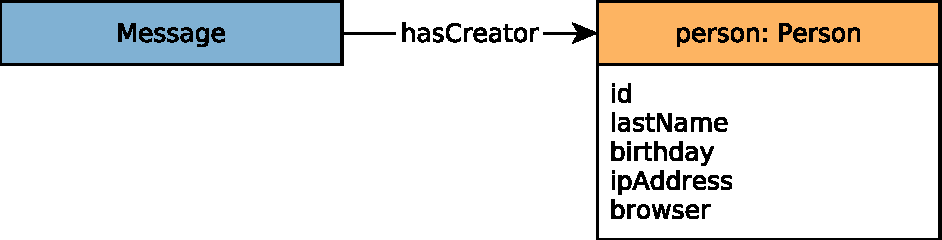
\includegraphics[scale=\patternscale,margin=0cm .2cm]{patterns/interactive-short-read-05}\hfill\vadjust{} \\ \hline
%
	desc. & Given a Message, retrieve its author.
 \\ \hline
%
	
%
	
		params &
		\innerCardVSpace{\begin{tabularx}{\attributeCardWidth}{|>{\paramNumberCell}c|>{\varNameCell}M|>{\typeCell}m{\typeWidth}|Y|} \hline
		$\mathsf{1}$ & Message.id
 & ID
 &  \\ \hline
		\end{tabularx}}\innerCardVSpace \\ \hline
	
%
	
		result &
		\innerCardVSpace{\begin{tabularx}{\attributeCardWidth}{|>{\resultNumberCell}c|>{\varNameCell}M|>{\typeCell}m{\typeWidth}|>{\resultOriginCell}c|Y|} \hline
		$\mathsf{1}$ & Message-hasCreator-\textgreater{}Person.id
 & ID
 & R &
				 \\ \hline
		$\mathsf{2}$ & Message-hasCreator-\textgreater{}Person.firstName
 & String
 & R &
				 \\ \hline
		$\mathsf{3}$ & Message-hasCreator-\textgreater{}Person.lastName
 & String
 & R &
				 \\ \hline
		\end{tabularx}}\innerCardVSpace \\ \hline
	
%
	%
	%
	%
	%
\end{tabularx}
\queryCardVSpace